\documentclass[journal]{IEEEtran}
\usepackage{listings}
\ifCLASSINFOpdf
  \usepackage[pdftex]{graphicx}
  \usepackage{amsfonts}
  % declare the path(s) where your graphic files are
  \graphicspath{{../pdf/}{../jpeg/}}
  % and their extensions so you won't have to specify these with
  % every instance of \includegraphics
  \DeclareGraphicsExtensions{.pdf,.jpeg,.png}
\else
  % or other class option (dvipsone, dvipdf, if not using dvips). graphicx
  % will default to the driver specified in the system graphics.cfg if no
  % driver is specified.
  \usepackage[dvips]{graphicx}
  % declare the path(s) where your graphic files are
  \graphicspath{{../eps/}}
  % and their extensions so you won't have to specify these with
  % every instance of \includegraphics
  \DeclareGraphicsExtensions{.eps}
\fi
\usepackage{graphics}
\usepackage{float}
\usepackage{caption}
\usepackage{url}
\hyphenation{op-tical net-works semi-conduc-tor}


\begin{document}

\title{Simulated Annealing aplicado ao TSP}


\author{Beatriz de Jesus Costa,
        ra104361@uem.br
        e~Bruna Stefany Batista Marques, ra103404@uem.br
}


% The paper headers



\maketitle


\begin{abstract}
With the increasing development of technology, it is necessary to use all available hardware resources to be able to keep up with such advances. Parallel programming is applied in order to use all available processor resources and, consequently, increase performance, decrease execution time, that is, improve results in several aspects. In order to make program parallelization possible, several tools have been created that make this possible, one of these tools is MPI. In this work, a sequential and a parallel version of the Simulated annealing algorithm applied to the Traveling Salesperson Problem will be implemented, using MPI, the results will be presented and discussed in relation to the performance of the versions.
\end{abstract}

\def\abstractname{Resumo}
\begin{abstract}
Com o crescente desenvolvimento da tecnologia, faz-se necessário a utilização de todos os recursos disponíveis de hardware para que seja possível acompanhar tais avanços. A programação paralela é aplicada visando utilizar todos os recursos disponíveis do processador e consequentemente, aumentar o desempenho, diminuir o tempo de execução, ou seja, melhorar os resultados em diversos aspectos. Para que seja possível a paralelização de programas, foram criadas diversas ferramentas que possibilitam isso, uma dessas ferramentas é o MPI. Neste trabalho será implementada uma versão sequencial e uma paralela do algoritmo Simulated Annealing aplicado ao Problema Caixeiro Viajante, utilizando MPI, os resultados serão apresentados e discutidos os resultados em relação ao desempenho das versões.
\end{abstract}


\begin{IEEEkeywords}
  simulated annealing, paralelisno, mpi, programação paralela, desempenho, tsp.
\end{IEEEkeywords}


\IEEEpeerreviewmaketitle



\section{Introdução}
\IEEEPARstart{D}esde muito tempo os profissionais da área da computação buscam uma melhoria na eficiência dos programas e aplicações. Com o crescimento das tecnologias, a necessidade de aplicações mais rápidas e eficientes se fizeram necessárias. Uma das alternativas para conseguir essa melhoria é a utilização de todos os recursos disponíveis nos computadores, como os processadores, desta forma, consequentemente, a utilização de programação paralela. Um programa paralelo é dividido em vários núcleos em um processador ou conjunto de processadores.

A computação paralela é a execução de muitas operações em uma única instância no tempo, ou seja, faz com que os núcleos disponíveis do  processador trabalhe de forma paralela. Explorar totalmente a computação paralela requer grande esforço e conhecimento do programador, no entanto, seus resultados geralmente tornam as aplicações que utilizam computação paralela muito mais eficientes. A principal motivação para executar as instruções do programa em paralelo é completar um
computação mais rápida \cite{lin}. Entre suas vantagens está a execução eficiente do código, uma vez que a programação paralela economiza tempo, permite a execução de aplicações em um menor tempo. Como consequência da execução eficiente do código, pode resolver problemas maiores. Além disso programação paralela vai além dos limites impostos pela computação sequencial, visto que pode utilizar muito mais recursos.

Quando um problema paralelo é resolvido, é esperada uma redução no tempo de execução que seja comensurável com a quantidade de recursos de processamento empregados para resolver o problema \cite{Kumar}. 

O MPI (Message Passing Interface) é um padrão de interface para a troca de mensagens em máquinas paralelas com memória distribuída em que uma aplicação é constituída por um ou mais processos que se comunicam, acionando-se funções para o envio e recebimento de mensagens entre os processos \cite{IGNACIO}. Basicamente, é uma biblioteca de troca de mensagens, desenvolvida para ser padrão, em ambientes de memória distribuída, em troca de mensagens e em computação paralela. Essa troca de mensagens é portável para qualquer arquitetura e tem aproximadamente 125 funções para
programação e ferramentas para se analisar a performance. No MPI, o paralelismo é explícito, ou seja, programador é responsável por identificar o paralelismo e implementar um algoritmo utilizando construções com o MPI.

O objetivo deste trabalho é implementar o algoritmo Simulated annealing aplicado ao Problema do Caixeiro Viajante (The Travelling Salesman Problem - TSP) em uma versão sequencial e em uma versão paralela, utilizando MPI. Além disso, também serão realizados experimentos com diferentes entrada de dados e diferentes números de processadores  e  analisar o desempenho dos algoritmos para essas entradas. Os algoritmos serão analisados por meio das medidas  \textit{speedup} e eficiência. 

\IEEEPARstart{A}

 
\hfill Novembro 11, 2020



\section{Problema}
\label{problema}
\subsection{Simulated Annealing}
O Simulated annealing (SA) ou Recozimento simulado, pode ser definido como uma técnica probabilística para aproximar o ótimo global de uma dada função. É uma meta-heurística para aproximar a otimização global em um grande espaço de busca para um problema de otimização que geralmente é utilizada quando o espaço de busca é discreto. 

O  algoritmo tem como base o processo de recozimento na física (annealing). Esse processo é conhecido como um processo térmico para obter estados de baixa energia de um sólido tendo duas etapas: aumentar a temperatura da etapa de banho de calor até um valor máximo ao qual o sólido derrete e diminuir cuidadosamente a temperatura do banho de calor até que as partículas se organizem no estado fundamental do sólido \cite{AARTS}. É importante que o resfriamento seja feito de forma suficientemente lenta para que o sólido não congele. Essa técnica é utilizada para aumentar o tamanho dos cristais do material utilizado e reduzir seus defeitos. 

O Simulated annealing pode ser aplicado em problemas de otimização computacional considerados muito difíceis, em que algoritmos exatos falham. O algoritmo geralmente atinge uma solução aproximada mas pode ser suficiente para muitos problemas. As aplicações do algoritmo a problemas são formulados por uma função objetivo sujeitas a várias restrições que se alteram em conforme o problema abordado. 

Segundo Aarts e Korst (1998), comparando o Simulated annealing  com a busca local, fica evidente que o Simulated annealing pode ser visto como uma generalização da pesquisa local, em que o Simulated annealing é melhor do que a busca local.

Um algoritmo Simulated Annealing repete um procedimento iterativo de geração de vizinho e segue as instruções de pesquisa que melhoram o valor da função objetivo. Enquanto explora a solução espaço, o método SA oferece a possibilidade de aceitar soluções de vizinhança piores de uma forma controlada maneira de escapar dos mínimos locais \cite{BOULEIMEN}.

O desempenho do algoritmo Simulated Annealing  é influenciado por fatores como critério de parada, a escolha do espaço de soluções factíveis, a função objetivo e a estrutura da escolha na vizinhança \cite{FUCHIGAMI}.

A ideia do algoritmo é começar com uma solução inicial qualquer, juntamente com uma temperatura, que deve ser alta. Uma função objetivo é definida com base no problema abordado, gerando uma solução S, que na primeira iteração será gerada a partir da solução inicial passada no começo do algoritmo. Enquanto a temperatura de entrada não atingir uma temperatura perto de zero,  soluções com mutações são geradas a partir da solução de inicial e caso essa nova solução for melhor que a solução anterior, ela vira a solução principal.  A cada  iteração, a temperatura é diminuída. Ao fim do algoritmo é retornada a melhor solução encontrada.

\subsection{Formulação SA}

\label{formulacao_seqsa}
\begin{table}[H]
    \centering
    \begin{tabular}{|c|}\hline
     \begin{lstlisting} 
    receba a temperatura T e um conjunto de
    solucao S inicial
    alpha = 0.99 e T_min = 0.00001
    f = funcao objetivo que varia em decorrencia
    do problema abordado
    faca:
        para i de 0 ate 100 faca:
            vizinho = S' (que e uma mutacao de S)
            delta = f(S') - f(S)
            se delta < 0 ou 
            exp((-delta)/T) * random(0,1) entao:
                S = S'
            fim-se
        fim-para
        T = T * alpha
    enquando T > T_min
    retorne S
    
\end{lstlisting} \\
         \hline
    \end{tabular}
    \label{tab:pseudo_seqSA}
\end{table}

\subsection{Simulated Annealing aplicado ao TSP}
O problema do Caixeiro viajante (TSP) é um problema NP-difícil em otimização combinatória, muito importante na área de ciência da computação e  está entre os problemas mais amplamente estudados, possuindo uma grande variedade de aplicações práticas.  Dado um conjunto de cidades, o problema consiste em definir um roteiro ótimo que visite todas as cidades com o menor custo possível. Embora uma solução ótima não possa ser alcançada, as soluções não ótimas se aproximam da otimização e mantêm o tempo de execução rápido \cite{Abdulkarim}.

O TSP é um problema muito importante, pois representa uma classe de problemas conhecida como NP-completo. Caso seja possível encontrar um algoritmo eficiente que encontre a solução ótima em um número polinomial de etapas para o TSP, então um algoritmo eficiente pode ser encontrado para todos os outros problemas na classe NP-completa, no entanto, até o momento \cite{GENG}.

A ideia do Simulated Annealing aplicado ao TSP é basicamente a mesma, primeiramente começamos com  uma solução inicial qualquer, neste caso, será um caminho a percorrer as cidades, juntamente com uma temperatura alta. A função objetivo é definida como a diferença da distância entre o caminho atual e um caminho vizinho, que é uma mutação do caminho atual. Enquanto a temperatura de entrada não atingir uma temperatura perto de zero,  soluções com mutações são geradas a partir da solução de inicial e caso essa nova solução for melhor que a solução anterior, ela vira a solução principal.  A cada  iteração, a temperatura é diminuída. Ao fim do algoritmo é retornada a melhor solução encontrada, que no caso do TSP será a menor distância entre as cidades.

Segundo Wang et all (2009). a ideia principal do algoritmo SA eficaz é baseada na informação entre duas cidades diferentes, e a informação vem das soluções ou passeios fechados obtidos pelo algoritmo SA simples na primeira etapa.

\subsection{Formulação TSP SA}
\label{formulacao_seqsatsp}
\begin{table}[H]
    \centering
    \begin{tabular}{|c|}\hline
     \begin{lstlisting} 
    receba a temperatura T e um caminho S
    alpha = 0.99 e T_min = 0.00001
    f = distancia entre as cidades
    do problema abordado
    faca:
        para i de 0 ate 100 faca:
            vizinho = S' (que e uma mutacao de S)
            delta = f(S') - f(S)
            se delta < 0 ou 
            exp((-delta)/T) * random(0,1) entao:
                S = S'
            fim-se
             se S* > S entao: //S* = melhor caminho
                S* = S
            fim-se
        fim-para
        T = T * alpha
    enquando T > T_min
    retorne s*
    
\end{lstlisting} \\
         \hline
    \end{tabular}
    \label{tab:pseudo_seq}
\end{table}

\section{Uma solução paralela}
A ideia do algoritmo paralelo do Simulated annealing aplicado ao TSP é praticamente a mesma da versão sequencial, a diferença é que o laço de repetição mais interno é dividido entre os processos e, ao final das iterações, o melhor caminho entre os processos é escolhido para ser o melhor caminho conhecido por todos.

As formas de paralelizar um problema são diversas, no entanto, a forma mais comum é baseado na divisão em várias partes para executá-las em paralelo e depois juntá-las. No entanto, essa abordagem não é geral para o problema do caixeiro viajante, sendo eficiente apenas para problemas de TSP com pelo menos centenas de cidades devido à sobrecarga de comunicação entre processadores, outra solução seria rodar vários processos, para todo o problema, em paralelo e comparar os resultados periodicamente \cite{MALEK}. 


Segundo os autores Jeong e Kim (1990), o procedimento do algoritmo pode ser descrito como: a configuração inicial é um passeio válido arbitrário que é definido como uma sequência de cidades; a energia de cada configuração corresponde à duração total do passeio; cada movimento em uma determinada temperatura envolve gerar uma nova configuração e permutar a ordem de visita das cidades, calcular a diferença de energia entre a nova e a antiga configuração, aceitar a nova configuração for menor que 0 ou com probabilidade $exp^{-delta/temperatura}$.

No algoritmo implementado nesse trabalho, primeiramente foi recebida uma temperatura T juntamente com um caminho S. Após isso o MPI foi inicializado, o valor da temperatura mínima e de alpha são fixos, o alpha é um das responsáveis pela diminuição da temperatura posteriormente. Após isso, a função objetivo é definida como a soma das distâncias entre as cidades do caminho. Uma barreira é colocada para garantir que todos os processos estejam prontos para começar o laço de repetição para a diminuição da temperatura. A fase de diminuir a temperatura começa e o algoritmo fará diversos indivíduos com mutações nos caminhos, calculará suas distâncias, irá comparar a distância do melhor caminho com a da melhor mutação e há ainda um ponto de sincronização em que o melhor caminho é enviado para todos os processadores, o laço se repetirá até que a temperatura atinja o valor mínimo.


\subsection{Formulação TSP SA Paralelo}
\label{formulacao_parsatsp}
\begin{table}[H]
    \centering
    \begin{tabular}{|c|}\hline
     \begin{lstlisting} 
    receba a temperatura T e um caminho S
    MPI_Init(&argv, &argc);
    MPI_Comm_size(MPI_COMM_WORLD, &world_size);
    MPI_Comm_rank(MPI_COMM_WORLD, &world_rank);
    alpha = 0.99 e T_min = 0.00001
    f = distancia entre as cidades
    do problema abordado
    MPI_Barrier(MPI_COMM_WORLD);
    faca:
        para i de 0 ate 100/world_size faca:
            vizinho = S' (que e uma mutacao de S)
            delta = f(S') - f(S)
            se delta < 0 ou 
            exp((-delta)/T) * random(0,1) entao:
                S = S'
            fim-se
            se S* > S entao: //S* = melhor caminho
                S* = S
            fim-se
        fim-para
        MPI_Allreduce(&S*, &S**, MPI_MIN...);
        T = T * alpha
    enquando T > T_min
    MPI_Barrier(MPI_COMM_WORLD);
    retorne S*
    MPI_Finalize();
    
\end{lstlisting} \\
         \hline
    \end{tabular}
    \label{tab:pseudo_seq}
\end{table}

\section{metodologia}
Ambos algoritmos foram construídos utilizando a linguagem de programação C. Para a implementação do algoritmo paralelo foi utilizada a biblioteca \textit{mpi}. Dessa biblioteca foram utilizadas as funções MPI\_Init(), MPI\_Comm\_size(), MPI\_Comm\_rank(), MPI\_Barrier() e MPI\_Allreduce(). Para a compilação do código paralelo foi utilizado o comando mpicc e para a execução foi utilizado o mpirun e especificado o número de processos desejado. Também foi necessário utilizar a opção "-lm" na compilação de ambos algoritmos para realizar a linkagem da biblioteca de matemática, que foi utilizada no código.

Foram utilizados grafos da biblioteca TSPLIB\footnote{http://elib.zib.de/pub/mp-testdata/tsp/tsplib/tsplib.html}  para as entradas dos algoritmos, sendo a entrada, que será mencionada posteriormente, small equivalente à nrw1379.tsp, a medium equivalente à pla7397.tsp e a large equivalente à brd14051.tsp. Nos algoritmos sequencial e paralelo, foram realizados testes e coletados os fitness(melhor resultado) e tempo de execução. Com o tempo de execução foi possível calcular o \textit{speedup} e a eficiência, tais resultados estão disponíveis na seção \ref{analise}. 

\subsection{Especificações Técnicas}
Os testes foram executados em um notebook Lenovo Ideapad 330. Este computador possui um processador Intel i5-8250U, o que siginifica que o processador é da oitava geração da Intel. O processador possui 8 CPUs, sendo 4 núcleos físicos e 4 virtuais, e frequência de 1,60GHz. Ele conta com 12 GB de memória RAM, 1 T de HD e 120 GB de SSD. Possui também uma GPU Integrada Intel UHD Graphics 620. 
O sistema operacional do computador é o Ubuntu 20.04.1 LTS, com versão GNOME 3.36.3. A versão do gcc instalada foi a 9.3.0. Os códigos foram executados utilizando o terminal padrão do sistema. Vale destacar uma alteração feita para otimização de memória do computador, que foi a mudança da configuração de memória SWAP de 60 para 10, isso significa que anteriormente, quando a memória RAM chegava em 40\% de sua capacidade, alguns pacotes de dados começavam a ser armazenados na memória SWAP, com a alteração essa taxa foi para 90\% da memória RAM, assim o sistema só utiliza o SWAP quando realmente precisa. Essa alteração otimiza o desempenho pois a memória SWAP é mais lenta que a memória RAM, já que é uma quantidade de memória física que é alocada para uso pelo sistema operacional.


\section{Análise e discussão}\label{analise}
As métricas escolhidas para analisar o desempenho das duas versões do algoritmo forram speedup e eficiência. Os resultados dos experimentos seguem nas seções abaixo.

Vale salientar que os resultados obtidos pelso algoritmos em relação ao menor caminho entre as cidades não foi o ideal, no entanto, foi próximo ao ideal.
\subsection{Speedup}\label{speedup}
\textit{Speedup} é uma métrica utilizada para analisar o desempenho entre dois sistemas, um sequencial e um paralelo, que resolvem o mesmo problema. É definido como a proporção do tempo de execução do melhor algoritmo sequencial pelo tempo gasto pelo algoritmo paralelo, em que ambos resolvem o mesmo problema. O \textit{speedup} é dado pela fórmula $TS/TP$, em que $TS$ é o tempo sequencial e $TP$ o tempo paralelo. O \textit{speedup} é considerado uma das melhores medidas para verificar se o desempenho do algoritmo paralelo é melhor que o sequencial.

Observando a figura \ref{fig:speedup} podemos notar que o \textit{speedup} para 1, 2 processadores atingiram valores bem perto do linear para todas entradas. No entanto, para 3 e principalmente 4 processadores, o valor fica um pouco distante. Um dos fatores que podem ter contribuído para isso seria que quanto mais processadores são usados, maior será o tempo de sincronização nos pontos que necessitam de sincronização, e também, maior a gerência de processos feita pelo MPI.
\begin{figure}[H]
    \centering
    \caption{Eficiência utilizando O0}
    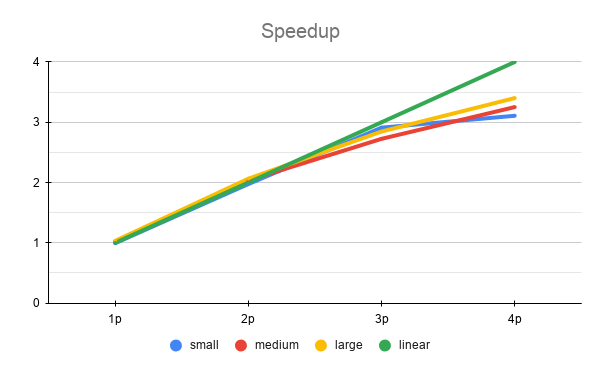
\includegraphics[width=3.7in]{imagens/speedup.png}
    \caption*{Fonte: Autoras, 2020}
    \label{fig:speedup}
\end{figure}

Outro fator que deve ser levado em conta é que um \textit{speedup} linear geralmente é muito difícil de alcançar por decorrência da contenção por recursos compartilhados, tempo necessário para se comunicar entre processadores e entre processos, e a incapacidade de estruturar o software para que um um número arbitrário de processadores possa ser mantido utilmente ocupado \cite{Eager}.

Vale também salientar que, como visto na seção \ref{problema}, o desempenho do Simulated Annealing  é influenciado pelo critério de parada,  escolha do espaço de soluções factíveis, função objetivo e a estrutura da escolha na vizinhança.

\subsection{Eficiência}
Eficiência métrica dada por $E(n) = S(n)/n$, em que S(n) diz respeito ao speedup e n o número de processadores.

\begin{figure}[H]
    \centering
    \caption{Eficiência utilizando O0}
    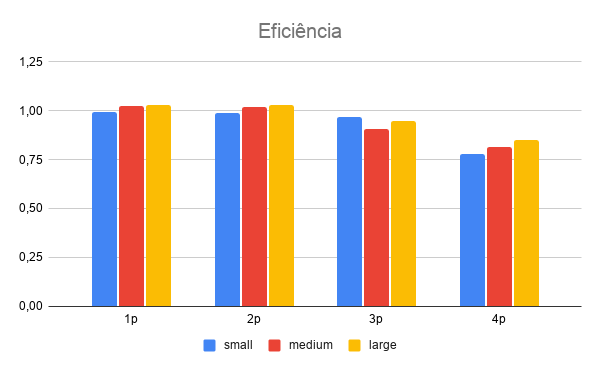
\includegraphics[width=3.7in]{imagens/eficiencia.png}
    \caption*{Fonte: Autoras, 2020}
    \label{fig:eficiencia}
\end{figure}

Segundo os autores Eager et all. se a eficiência de um algoritmo permanecer em 1 conforme os processadores são adicionados, temos um \textit{speedup} linear. Ao observar o gráfico de eficiência contido na figura \ref{fig:eficiencia} e com base na definição acima, podemos notar que paras as entradas média e grande, nos processadores 1 e 2, um \textit{speedup} linear foi obtido. Ao observar os resultados para 3 processadores, podemos notar pela eficiência que para as entradas pequena e grande o \textit{speedup} foi quase linear. No entanto, para 4 processadores, o \textit{spedup} foi um pouco longe do linear, o que se confirma o resultado mostrado na figura \ref{fig:speedup}

\section{Conclusões e trabalhos futuros}
Com a realização deste trabalho foi possível adquirir e aprofundar conhecimentos sobre programação paralela e aprender sabre algoritmos clássicos da computação, como o TSP e o Simulated annealing. Também foi possível aprender como o MPI funciona e suas principais funções. Fomos capazes de observar que a paralelização de problemas é muito necessária na atualidade e que existem diversas ferramentas que possibilitam isso.

Sobre os resultados, podemos concluir que o código paralelo foi melhor que o sequencial em questões de tempo de execução.Os resultados poderiam ser melhorados tomando uma abordagem diferente ou alterando o modo em que são feitos os pontos de sincronização dos processos no código.

As configurações e especificações da máquina utilizada para as execuções podem ter interferido nos resultados finais.

Para trabalhos futuros pretende-se um aprofundamento nos estudos sobre os tópicos abordados, para que seja possível remodelar o problema para atingir resultados melhores. Também almeja-se realizar experimentos com quantidades diferentes de temperatura e entradas diferentes.

\section*{Agradecimentos}
Ao professor pelo ensino que possibilitou a realização deste trabalho e aos colegas por todo apoio e ajuda.



\ifCLASSOPTIONcaptionsoff
  \newpage
\fi


\begin{thebibliography}{1}

\bibitem{Kumar} KUMAR, Vijay P.. ; GUPTA, Anshul. Analyzing scalability of parallel algorithms and architectures. Journal of parallel and distributed computing, v. 22, n. 3, p. 379-391, 1994.

\bibitem{AARTS}
AARTS, Emile; KORST, Jan. Simulated annealing and Boltzmann machines. 1988.
  
 \bibitem{BOULEIMEN} BOULEIMEN, KLEIN; LECOCQ, HOUSNI. A new efficient simulated annealing algorithm for the resource-constrained project scheduling problem and its multiple mode version. European journal of operational research, v. 149, n. 2, p. 268-281, 2003.
 
 \bibitem{FUCHIGAMI} FUCHIGAMI, Helio Yochihiro. Proposição de algoritmo simulated annealing para programação em flow shops paralelos proporcionais com tempos de setup explícitos. Revista Produção Online, v. 14, n. 3, p. 997-1023, 2014.
 
 \bibitem{Abdulkarim}Abdulkarim, Haider and Alshammari, Ibrahim Fadhil. (2015). Comparison of Algorithms for Solving Traveling Salesman Problem. International Journal of Engineering and Advanced Technology. ISSN. 2249 – 8958. 
 
 \bibitem{GENG} GENG, Xiutang et al. Solving the traveling salesman problem based on an adaptive simulated annealing algorithm with greedy search. Applied Soft Computing, v. 11, n. 4, p. 3680-3689, 2011.
 
 \bibitem{WANG} WANG, Zicheng; GENG, Xiutang; SHAO, Zehui. An effective simulated annealing algorithm for solving the traveling salesman problem. Journal of Computational and Theoretical Nanoscience, v. 6, n. 7, p. 1680-1686, 2009.
 
 \bibitem{IGNACIO} IGNÁCIO, Aníbal Alberto Vilcapona; FERREIRA FILHO, Virgílio José Martins. MPI: uma ferramenta para implementação paralela. Pesquisa Operacional, v. 22, n. 1, p. 105-116, 2002.
 
 \bibitem{lin} LIN, Calvin et al. Principles of parallel programming. Pearson Education India, 2008.
 
 \bibitem{MALEK} MALEK, Miroslaw et al. Serial and parallel simulated annealing and tabu search algorithms for the traveling salesman problem. Annals of Operations Research, v. 21, n. 1, p. 59-84, 1989.
 
 \bibitem{JEONG} JEONG, Chang-Sung; KIM, M. H. Fast parallel simulated annealing for traveling salesman problem. In: 1990 IJCNN International Joint Conference on Neural Networks. IEEE, 1990. p. 947-953.
 
\bibitem{Eager}D. L. Eager, J. Zahorjan and E. D. Lazowska, "Speedup versus efficiency in parallel systems," in IEEE Transactions on Computers, vol. 38, no. 3, pp. 408-423, March 1989, doi: 10.1109/12.21127.


\end{thebibliography}





\end{document}


